
\clearpage
\section{Calcolo Combinatorio}
\subsection{Prodotto Cartesiano}

Si considerino $k$ insiemi finiti, $A_1, \dots, A_k$, non necessariamente distinti.
\\\\Si definisce \textbf{prodotto cartesiano} $A^{(k)} = A_1 \times \dots \times A_k$ un insieme costituito dalle $k$-ple ordinate in cui il primo elemento appartiene a $A_1$, il secondo a $A_2$ e così via.
\\\\Siccome il primo elemento si può scegliere in $|A_1|$ modi, il secondo in $|A_2|$ e così via, avremo:
    \[
    |A^{(k)}| = \prod_{i=1}^{k} |A_i|
    \]
Questa è la relazione fondamentale del calcolo combinatorio, dalla quale molte altre formule di conteggio derivano.

\subsection{Disposizioni Semplici (k-ple ordinate senza ripetizione)}

Abbiamo un insieme $A$ con $n$ elementi. Vogliamo capire quante stringhe ordinate di lunghezza $k$ possiamo formare con la condizione che ogni elemento di $A$ può apparire una ed una sola volta.

\begin{esempio}
	C'è una gara con 8 atleti ($n=8$). Quanti possibili podi (oro, argento, bronzo) possiamo avere ($k=3$)?
\end{esempio}

Il ragionamento è il seguente:
\begin{enumerate}
	\item \textbf{Scegliamo il primo elemento:} abbiamo $n$ possibili scelte.
	\item \textbf{Scegliamo il secondo elemento:} abbiamo $n-1$ possibili scelte (perché non possiamo riprendere l'elemento scelto in precedenza).
	\item \textbf{Scegliamo il terzo elemento:} abbiamo $n-2$ scelte.
	\item[\dots]
	\item \textbf{Scegliamo il $k$-esimo elemento:} abbiamo $n - (k-1) = n - k + 1$ scelte.
\end{enumerate}

Applicando la regola del prodotto, il numero totale di stringhe possibili, per ogni $k \le n$, è:
\[ n \cdot (n-1) \cdot (n-2) \cdot \dots \cdot (n - k + 1) \]
che possiamo scrivere in modo compatto come:
\[ \prod_{i=0}^{k-1} (n-i) \]
Questa formula viene quasi sempre scritta in una forma ancora più compatta usando i fattoriali. Ricorda che $n! = n \cdot (n-1) \cdot \dots \cdot 2 \cdot 1$.
\\\\La formula delle \textbf{Disposizioni Semplici} $D_{n,k}$ è:
\[ D_{n,k} = \frac{n!}{(n-k)!} \]

\paragraph{Perché funziona?}
Espandendo i fattoriali si osserva che i termini si semplificano:
\[ \frac{n!}{(n-k)!} = \frac{n \cdot (n-1) \cdot \dots \cdot (n-k+1) \cdot (n-k)!}{(n-k)!} \]
Tutti i termini da $(n-k)$ in giù si annullano, lasciando esattamente la formula di partenza: $n \cdot (n-1) \cdot \dots \cdot (n-k+1)$.

\begin{esempio}[Risoluzione Esempio del Podio]
Con $n=8$ atleti e $k=3$ posizioni sul podio:
\[ \text{Numero di podi possibili} = 8 \cdot 7 \cdot 6 = 336 \]
Usando la formula con i fattoriali:
\[ D_{8,3} = \frac{8!}{(8-3)!} = \frac{8!}{5!} = \frac{8 \cdot 7 \cdot 6 \cdot 5!}{5!} = 8 \cdot 7 \cdot 6 = 336 \]
\end{esempio}

\begin{osservazione}
	Il caso speciale in cui $k=n$ prende il nome di \textbf{permutazione}. In questo caso, vogliamo contare le stringhe di lunghezza $n$ usando \emph{tutti} gli $n$ elementi, senza ripetizioni. In altre parole, stiamo contando in quanti modi diversi possiamo ordinare (o mettere in fila) tutti gli elementi dell'insieme.
\end{osservazione}

La formula per le permutazioni di $n$ elementi, indicata con $P_n$, è:
\[ P_n = D_{n,n} = \frac{n!}{(n-n)!} = \frac{n!}{0!} = n! \]
(ricordando che per definizione $0! = 1$).

\begin{esempio}
In quanti modi diversi posso disporre 3 libri ($n=3$) su uno scaffale?
\[ P_3 = 3! = 3 \cdot 2 \cdot 1 = 6 \]
\end{esempio}

\subsection{Disposizioni con Ripetizione (k-ple ordinate con ripetizione)}

Abbiamo un insieme $A$ con $n$ elementi distinti. Vogliamo sempre formare delle "stringhe" (sequenze ordinate) di lunghezza $k$.
A differenza del caso precedente, ora ogni elemento può essere usato \textbf{più di una volta}.

Il ragionamento è il seguente:
\begin{itemize}
    \item Per la scelta del primo elemento abbiamo $n$ possibilità.
    \item Per la scelta del secondo elemento abbiamo ancora $n$ possibilità (poiché la ripetizione è permessa).
    \item \dots
    \item Per la scelta del $k$-esimo elemento, abbiamo sempre $n$ possibilità.
\end{itemize}

Applicando il principio fondamentale del calcolo combinatorio (la regola del prodotto), otteniamo:
\[ \underbrace{n \cdot n \cdot n \cdot \dots \cdot n}_{k \text{ volte}} \]
Questo è, per definizione, la potenza $k$-esima di $n$.
\[ n^k \]

\begin{osservazione}
Questo risultato non è altro che la cardinalità del prodotto cartesiano dell'insieme $A$ con se stesso per $k$ volte. Se $A^{(k)} = A \times A \times \dots \times A$ ($k$ volte), allora $|A^{(k)}| = |A|^k = n^k$.
\end{osservazione}

% Da inserire di seguito al codice precedente in chapters/1.tex

\subsection{Combinazioni Semplici (Sottoinsiemi non ordinati)}

Prima abbiamo visto il concetto di disposizione. Qual è la differenza con la parola ``combinazione''?

Le \textbf{combinazioni} $C_{n,k}$ di $n$ "elementi presi a gruppi di $k$" contano in quanti modi si possono scegliere $k$ elementi da un insieme di $n$ elementi, \textbf{senza tenere conto dell'ordine}. 

Questo significa che le combinazioni sono sempre minori o uguali alle disposizioni, perché gruppi ordinati come $(1,2,3)$, $(3,2,1)$ e $(2,1,3)$ ``collassano'' in un unico sottoinsieme non ordinato $\{1,2,3\}$.
\\\\Deriviamo la formula:
\\Iniziamo calcolando tutti i possibili gruppi ordinati di $k$ elementi presi da $n$. Questa è esattamente la formula delle disposizioni semplici che abbiamo già visto:
\[ D_{n,k} = \frac{n!}{(n-k)!} \]

\paragraph{Rimuoviamo la ridondanza}
Prendiamo uno specifico gruppo di $k$ elementi, ad esempio il sottoinsieme $\{1, 2, 3\}$ (con $k=3$). Quante volte appare questo gruppo nella nostra lista di \textit{disposizioni}? Appare in tutte le sue possibili permutazioni:
\begin{itemize}
    \item $(1, 2, 3)$
    \item $(1, 3, 2)$
    \item $(2, 1, 3)$
    \item $(2, 3, 1)$
    \item $(3, 1, 2)$
    \item $(3, 2, 1)$
\end{itemize}
Tutte queste $3! = 6$ sequenze ordinate, dal punto di vista delle combinazioni (dove l'ordine non conta), sono la \textbf{stessa e unica cosa}.

In generale, per un qualsiasi gruppo di $k$ elementi, esistono $k!$ modi di ordinarli. Questo significa che, nella nostra lista iniziale di disposizioni, ogni combinazione unica è stata contata $k!$ volte di troppo. Per ottenere il numero corretto di combinazioni, dobbiamo quindi dividere il numero totale di disposizioni per questo fattore di ridondanza.
\\\\La formula per le \textbf{Combinazioni Semplici}, indicata anche con il \textbf{coefficiente binomiale} $\binom{n}{k}$, è:
\[ C_{n,k} = \binom{n}{k} = \frac{D_{n,k}}{k!} = \frac{n!}{k!(n-k)!} \]

\subsubsection{Esempi Pratici}
\begin{itemize}
    \item \textbf{SuperEnalotto:} Bisogna scegliere 6 numeri da un insieme di 90 ($n=90, k=6$). L'ordine con cui vengono estratti non influenza la vincita. Quante sono le possibili sestine?
    \[ \binom{90}{6} = \frac{90!}{6!(90-6)!} = \frac{90!}{6! \cdot 84!} = 622.614.630 \]
    
    \item \textbf{Mano di Poker:} Quante diverse mani di 5 carte ($k=5$) si possono ricevere da un mazzo di 52 ($n=52$)? L'ordine in cui si ricevono le carte non cambia la mano.
    \[ \binom{52}{5} = \frac{52!}{5!(52-5)!} = \frac{52!}{5! \cdot 47!} = 2.598.960 \]
\end{itemize}

\subsection{Insieme delle parti di un insieme finito}

Si consideri un insieme $A$ con $n$ elementi.
\\L'insieme delle parti $\mathcal{P}(A)$ di $A$ è l'insieme di tutti i possibili sottoinsiemi di $A$.
Negli insiemi ovviamente l'ordinamento non conta, per cui il numero di sottoinsiemi $k$-dimensionali di $A$ è:
    \[ \binom{n}{k} \]
Siccome tanto l'insieme vuoto ($0$-dimensionale) quanto $A$ ($n$-dimensionale) sono sottoinsiemi di $A$, avremo:
    \[ |\mathcal{P}(A)| = \sum_{k=0}^{n} \binom{n}{k} = 2^n \]

\begin{esempio}
Un giocatore estrae (senza reinserimento) 5 carte da un mazzo di carte da poker (contenente le carte dal 7 all’asso, per un totale di $8 \times 4 = 32$ carte).
Calcolare le seguenti probabilità:
\begin{enumerate}
    \item Coppia di assi e coppia qualsiasi;
    \item Almeno tre assi;
    \item Un tris qualsiasi (ma non un full nè un poker);
    \item Colore di picche o colore qualsiasi.
\end{enumerate}

\paragraph{Soluzione 1) Coppia di assi e coppia qualsiasi}

Per calcolare la probabilità di un evento si utilizza la formula:
\[
\text{Probabilità} = \frac{\text{Numero di Mani Favorevoli}}{\text{Numero Totale di Mani Possibili}}
\]

Per prima cosa, calcoliamo il denominatore, ovvero quante combinazioni di 5 carte si possono estrarre da un mazzo di 32, senza reinserimento e senza considerare l'ordine. Il numero totale di mani possibili è dato da:
\[
\binom{32}{5} = \frac{32!}{5!(32-5)!} = \frac{32 \cdot 31 \cdot 30 \cdot 29 \cdot 28}{5 \cdot 4 \cdot 3 \cdot 2 \cdot 1} = \mathbf{201.376} \text{ mani possibili}
\]

Ora calcoliamo il numeratore, ovvero in quanti modi possiamo ottenere una mano con una coppia di assi e un'altra coppia qualsiasi. Suddividiamo il problema in passaggi:

\begin{enumerate}
    \item \textbf{Scegliamo la coppia di assi:} ci sono 4 assi nel mazzo e dobbiamo sceglierne 2:
    \[ \binom{4}{2} = \frac{4!}{2!2!} = 6 \text{ modi} \]
    
    \item \textbf{Scegliamo il valore della seconda coppia:} il mazzo ha 8 valori di carte (7, 8, 9, 10, J, Q, K, A). Avendo già scelto gli assi come valore per la prima coppia, rimangono 7 valori possibili per la seconda coppia:
    \[ \binom{7}{1} = 7 \text{ modi} \]
    
    \item \textbf{Scegliamo le due carte per la seconda coppia:} per il valore scelto (ad esempio, i Re), ci sono 4 carte di quel valore nel mazzo. Dobbiamo sceglierne 2:
    \[ \binom{4}{2} = 6 \text{ modi} \]
    
    \item \textbf{Scegliamo la quinta carta:} questa carta non può essere né un asso né del valore della seconda coppia, altrimenti avremmo un full. Le carte totali sono 32.
    \begin{itemize}
        \item Togliamo i 4 assi: $32 - 4 = 28$.
        \item Togliamo le 4 carte del valore della seconda coppia: $28 - 4 = 24$.
    \end{itemize}
    Dobbiamo quindi scegliere una carta tra le restanti 24:
    \[ \binom{24}{1} = 24 \text{ modi} \]
\end{enumerate}

Il numero totale di mani favorevoli si ottiene moltiplicando i risultati di ogni passaggio:
\[
\text{Casi Favorevoli} = \binom{4}{2} \cdot \binom{7}{1} \cdot \binom{4}{2} \cdot \binom{24}{1} = 6 \cdot 7 \cdot 6 \cdot 24 = \mathbf{6.048} \text{ mani}
\]

Ora possiamo unire i due risultati per calcolare la probabilità:
\[
\text{Probabilità} = \frac{\text{Casi Favorevoli}}{\text{Casi Possibili}} = \frac{6.048}{201.376} \approx 0,030033
\]
La probabilità di estrarre una coppia di Assi e un'altra coppia qualsiasi è quindi di circa il \textbf{3,00\%}.


\paragraph{Soluzione 2) Almeno tre assi}
L'evento "almeno tre assi" si realizza se si verifica uno dei due eventi mutuamente esclusivi: "esattamente 3 assi" oppure "esattamente 4 assi". Calcoliamo separatamente le probabilità.

\subparagraph{Probabilità di estrarre esattamente 3 assi}
Questa mano è composta da 3 assi e 2 carte che non sono assi.
\begin{itemize}
    \item Scegliamo 3 assi dai 4 disponibili nel mazzo:
    \[ \binom{4}{3} = 4 \text{ modi} \]
    \item Scegliamo le altre 2 carte dalle 28 carte rimanenti che non sono assi:
    \[ \binom{28}{2} = \frac{28!}{2! \cdot 26!} = \frac{28 \cdot 27}{2} = 378 \text{ modi} \]
\end{itemize}
Moltiplichiamo i risultati per trovare il numero di mani favorevoli (che include anche il full house):
\[ \text{Casi Favorevoli (3 assi)} = 4 \cdot 378 = \mathbf{1.512} \text{ mani} \]

\subparagraph{Probabilità di estrarre esattamente 4 assi (Poker d'assi)}
Questa mano è composta da 4 assi e 1 carta qualsiasi che non sia un asso.
\begin{itemize}
    \item Scegliamo 4 assi dai 4 disponibili:
    \[ \binom{4}{4} = 1 \text{ modo} \]
    \item Scegliamo 1 carta dalle 28 rimanenti:
    \[ \binom{28}{1} = 28 \text{ modi} \]
\end{itemize}
Moltiplichiamo i risultati:
\[ \text{Casi Favorevoli (4 assi)} = 1 \cdot 28 = \mathbf{28} \text{ mani} \]

\subparagraph{Probabilità totale}
Per ottenere la probabilità di estrarre "almeno tre assi", sommiamo le mani favorevoli dei due casi e le dividiamo per il totale delle mani possibili.
\begin{itemize}
    \item \textbf{Totale mani favorevoli}: $1.512 \text{ (3 assi)} + 28 \text{ (4 assi)} = \mathbf{1.540}$
    \item \textbf{Probabilità}: 
    \[ P(\text{almeno 3 assi}) = \frac{1.540}{201.376} \approx 0,007647 \]
\end{itemize}
La probabilità è quindi di circa lo \textbf{0,76\%}.

\vspace{1cm} % Aggiunge uno spazio verticale per separare i ragionamenti

\hrule % Aggiunge una linea di separazione

\vspace{1cm}

\subparagraph{Approfondimento: Probabilità di 3 assi escludendo il Full House}
Ora calcoliamo la probabilità di estrarre una mano con esattamente 3 assi e due carte di valore diverso tra loro (del tipo AAAXY).

\begin{enumerate}
    \item \textbf{Scegliamo i 3 assi:} Dal mazzo che contiene 4 assi, dobbiamo sceglierne 3. Il numero di modi per farlo è:
    \[ \binom{4}{3} = \mathbf{4} \]
    
    \item \textbf{Scegliamo le restanti due carte (X e Y):} Queste devono soddisfare due condizioni:
    \begin{itemize}
        \item Non devono essere assi.
        \item Non devono avere lo stesso valore (per evitare una coppia, che formerebbe un full house AAAXX).
    \end{itemize}
    
    Il procedimento è il seguente:
    \begin{itemize}
        \item \textbf{Scegliamo i due valori diversi per X e Y:} tolti gli assi, rimangono 7 valori possibili (7, 8, 9, 10, J, Q, K). Di questi ne dobbiamo scegliere 2:
        \[ \binom{7}{2} = \frac{7!}{2!5!} = 21 \text{ coppie di valori possibili} \]
        (es. \{Re, Donna\}, \{7, 9\}, ecc.).
        
        \item \textbf{Scegliamo il seme per la prima carta (X):} per il primo valore scelto (es. Re), ci sono 4 semi disponibili:
        \[ \binom{4}{1} = \mathbf{4} \]
        
        \item \textbf{Scegliamo il seme per la seconda carta (Y):} anche per il secondo valore (es. Donna), ci sono 4 semi disponibili:
        \[ \binom{4}{1} = \mathbf{4} \]
    \end{itemize}
    Per ottenere il numero totale di modi per scegliere le carte X e Y, moltiplichiamo i risultati di questi tre sottogruppi:
    \[ \text{Modi per scegliere X e Y} = \binom{7}{2} \cdot \binom{4}{1} \cdot \binom{4}{1} = 21 \cdot 4 \cdot 4 = \mathbf{336} \]
    
    \item \textbf{Calcolo finale delle mani favorevoli:} adesso moltiplichiamo questo risultato per il numero di modi per scegliere gli assi:
    \[ \text{Mani favorevoli (AAAXY)} = 4 \text{ (modi per assi)} \cdot 336 \text{ (modi per X e Y)} = \mathbf{1.344} \]
    
    \item \textbf{Calcolo della probabilità:}
    \[ P(\text{Tris d'assi, non full}) = \frac{1.344}{201.376} \approx 0,006674 \]
\end{enumerate}
La probabilità di estrarre esattamente 3 assi senza avere un full house è quindi di circa lo \textbf{0,67\%}.

\paragraph{Soluzione 3) Un tris qualsiasi (ma non un full nè un poker)}
L'obiettivo è calcolare la probabilità di ottenere una mano di tipo ZZZXY, dove Z, X e Y sono tre valori distinti. Questo esclude il full (ZZZXX) e il poker (ZZZZX).

\begin{enumerate}
    \item \textbf{Scegliamo il valore del tris (Z):}
    Ci sono 8 valori possibili nel mazzo (dal 7 all'Asso). Dobbiamo sceglierne uno per il nostro tris.
    \[ \text{Scelta del valore:} \binom{8}{1} = 8 \text{ modi} \]

    \item \textbf{Scegliamo i 3 semi per quel valore:}
    Per il valore scelto (ad esempio, il Re), ci sono 4 semi. Dobbiamo sceglierne 3.
    \[ \text{Scelta dei semi:} \binom{4}{3} = 4 \text{ modi} \]

    \item \textbf{Scegliamo le ultime due carte (X e Y):}
    Le due carte rimanenti devono avere valori diversi sia dal tris sia tra di loro.
    \begin{itemize}
        \item \textbf{Scegliere i 2 valori diversi:} Restano 7 valori disponibili nel mazzo (8 totali meno quello usato per il tris). Ne dobbiamo scegliere 2.
        \[ \text{Scelta dei valori:} \binom{7}{2} = \frac{7 \cdot 6}{2} = 21 \text{ modi} \]
        
        \item \textbf{Scegliere il seme per la prima carta (X):} Per il primo dei due valori scelti, ci sono 4 semi disponibili.
        \[ \text{Scelta del seme di X:} \binom{4}{1} = 4 \text{ modi} \]
        
        \item \textbf{Scegliere il seme per la seconda carta (Y):} Anche per il secondo valore scelto, ci sono 4 semi disponibili.
        \[ \text{Scelta del seme di Y:} \binom{4}{1} = 4 \text{ modi} \]
    \end{itemize}
\end{enumerate}

Per calcolare il numero totale di mani favorevoli, moltiplichiamo il numero di opzioni per ogni passaggio:
\begin{align*}
\text{Mani favorevoli} &= (\text{Scelta valore tris}) \times (\text{Scelta semi tris}) \times (\text{Scelta valori X, Y}) \\
                      &\quad \times (\text{Scelta seme X}) \times (\text{Scelta seme Y}) \\
\text{Mani favorevoli} &= \binom{8}{1} \cdot \binom{4}{3} \cdot \binom{7}{2} \cdot \binom{4}{1} \cdot \binom{4}{1} \\
                      &= 8 \times 4 \times 21 \times 4 \times 4 = \mathbf{10.752}
\end{align*}

\subsubsection*{2. Calcolo della Probabilità}
Dividiamo il numero di mani favorevoli per il numero totale di mani possibili (201.376).
\[
\text{Probabilità} = \frac{10.752}{201.376} \approx 0,05339...
\]
Convertendo in percentuale, la probabilità è di circa il \textbf{5,34\%}.


\paragraph{Soluzione 4) Colore di Picche o Colore Qualsiasi}

L'evento "Colore di Picche" è un caso specifico dell'evento più generale "Colore Qualsiasi". Pertanto, la probabilità dell'unione "Colore di Picche o Colore Qualsiasi" è semplicemente la probabilità dell'evento "Colore Qualsiasi".

Per chiarezza, calcoliamo prima il caso specifico e poi lo generalizziamo.

\subsubsection*{Colore di Picche}
Un "colore di picche" significa che tutte e 5 le carte estratte devono essere di picche.

\begin{itemize}
    \item \textbf{Carte disponibili:} Nel mazzo di 32 carte, ci sono 8 carte di picche (7, 8, 9, 10, J, Q, K, A).
    \item \textbf{Mani favorevoli:} Dobbiamo scegliere 5 di queste 8 carte. Utilizziamo le combinazioni:
    \[
    \binom{8}{5} = \frac{8!}{5!(8-5)!} = \frac{8!}{5!3!} = \frac{8 \times 7 \times 6}{3 \times 2 \times 1} = \mathbf{56}
    \]
    Ci sono esattamente \textbf{56} mani possibili che costituiscono un colore di picche.
\end{itemize}

La probabilità di questo evento specifico è:
\[
P(\text{Colore di Picche}) = \frac{56}{201.376} \approx 0,000278 \approx \mathbf{0,028\%}
\]

\subsubsection*{Colore Qualsiasi}
Un "colore qualsiasi" (o \textit{flush}) significa ottenere 5 carte dello stesso seme, non importa quale. 
\\\\\textbf{Mani favorevoli:} il calcolo che abbiamo fatto per il seme di picche è identico per qualsiasi altro seme (cuori, quadri, fiori), poiché ogni seme ha 8 carte. Il numero totale di mani favorevoli per un colore qualsiasi è la somma dei casi per ciascun seme:
    \[
    \text{Mani favorevoli (Colore Qualsiasi)} = 56 (\text{picche}) + 56 (\text{cuori}) + 56 (\text{quadri}) + 56 (\text{fiori})
    \]
    \[
    = 56 \times 4 = \mathbf{224}
    \]

La probabilità di ottenere un colore qualsiasi è quindi:
\[
P(\text{Colore Qualsiasi}) = \frac{224}{201.376} \approx 0,001112 \approx \mathbf{0,11\%}
\]
\end{esempio}

\newpage


\section*{Dagli Eventi Equiprobabili a Quelli Non Equiprobabili: Il mondo reale}

\subsection*{1. Spazi Campione Discreti}

Iniziamo definendo il nostro campo di gioco: uno spazio campione \(\Omega\) discreto, ovvero un insieme di risultati possibili che possiamo contare o elencare (finito o numerabile).
\\\\
Il passo fondamentale che compiamo ora è rimuovere l'ipotesi che tutti gli eventi elementari siano equiprobabili. Questo ci permette di modellare scenari più realistici, come il lancio di un dado truccato o una moneta sbilanciata.
\\\\
Anche in assenza di equiprobabilità, la definizione fondamentale di probabilità rimane valida attraverso l'approccio frequentista. Questo metodo si basa sull'osservazione sperimentale:
\begin{itemize}
    \item Si considera un evento A (un sottoinsieme di \(\Omega\)) e si ripete l'esperimento \(n\) volte.
    \item Si conta il numero di volte \(n_A\) in cui l'evento A si verifica.
    \item La frequenza relativa di A è il rapporto: \( f_n(A) = \frac{n_A}{n} \).
    \item La \textbf{Probabilità P(A)} è il valore a cui questa frequenza tende a stabilizzarsi all'aumentare infinito del numero di prove (\(n \to \infty\)).
\end{itemize}

Nel modello equiprobabile, ogni risultato ha la stessa identica chance di verificarsi. Qui, il calcolo della probabilità si basa su un principio semplice: il conteggio.
\\\\
La probabilità di un evento A è data dal rapporto tra il numero di casi favorevoli e il numero di casi possibili:
\[ P(A) = \frac{|A|}{|\Omega|} \]
\\
Di conseguenza, se ripetiamo l'esperimento \(n\) volte, ci aspettiamo che A si verifichi un numero di volte approssimativamente pari a \( n \cdot P(A) = n \cdot \frac{|A|}{|\Omega|} \).

\begin{esempio}[Lancio di un dado non truccato]
    \begin{itemize}
        \item \(\Omega = \{1, 2, 3, 4, 5, 6\}\), quindi \(|\Omega| = 6\).
        \item Evento A = "Esce un numero pari" = \(\{2, 4, 6\}\), quindi \(|A| = 3\).
        \item \(P(A) = \frac{3}{6} = 0.5\).
        \item Su 1000 lanci, ci aspettiamo circa \(1000 \cdot 0.5 = 500\) risultati pari.
    \end{itemize}
\end{esempio}
In questo mondo, la "misura" o il "peso" di un evento coincide con la sua cardinalità, ovvero il numero di elementi che contiene.

\subsection*{2. Pesi}

Quando gli eventi elementari non sono equiprobabili, ogni risultato possiede un suo "peso" intrinseco: la sua probabilità individuale. La cardinalità di un evento non è più sufficiente per determinarne la probabilità.

La differenza fondamentale è che il numero di occorrenze \(n_A\) non dipende più solo da quanti elementi ci sono in A, ma da quanto sono probabili quegli elementi.

\begin{esempio}[ Lancio di un dado non truccato]
    Supponiamo che le probabilità siano: \(P(6) = 50\%\), mentre \(P(1) = P(2) = P(3) = P(4) = P(5) = 10\%\).
    \begin{itemize}
        \item Evento A = "Esce un numero pari" = \(\{2, 4, 6\}\).
        \item La vecchia formula basata sul conteggio darebbe un errato \(P(A) = 3/6 = 0.5\).
    \end{itemize}
    Il metodo corretto è sommare i pesi (le probabilità) dei singoli risultati che compongono l'evento:
    \[ P(A) = P(2) + P(4) + P(6) = 0.1 + 0.1 + 0.5 = 0.7 \]
    La probabilità reale è del 70\%. Su 1000 lanci, ci aspetteremmo circa \(1000 \cdot 0.7 = 700\) risultati pari, un valore molto diverso dai 500 del dado non truccato.
\end{esempio}

Il passaggio a eventi non equiprobabili segna un cambiamento cruciale nel metodo:
\begin{itemize}
    \item Le tecniche di calcolo combinatorio non sono più sufficienti da sole per calcolare la probabilità.
    \item Non possiamo più limitarci a calcolare \(\frac{\text{casi favorevoli}}{\text{casi totali}}\). Dobbiamo prima conoscere la probabilità (il "peso") di ogni singolo risultato elementare e poi sommare i pesi di tutti i risultati che formano il nostro evento.
\end{itemize}
In sintesi, si passa da un modello dove \textbf{"probabilità è contare"} a un modello più generale e potente dove \textbf{"probabilità è pesare e sommare"}.


\begin{esempio}[Il Dado Truccato]

Supponiamo di avere un dado, ma questa volta truccato in modo che 5 volte su 6 esca il risultato 1.

Si lanci il dado un’unica volta, per cui lo spazio campione è \(\Omega = \{1, 2, 3, 4, 5, 6\}\).
Definiamo due eventi:
\begin{itemize}
    \item \(A = \{\text{Il risultato è pari}\} = \{2, 4, 6\}\)
    \item \(B = \{\text{Il risultato è dispari}\} = \{1, 3, 5\}\)
\end{itemize}

Chiamiamo \(n_i\) il numero delle volte che esce il risultato \(i\) su \(n\) prove.
\\\\La somma delle occorrenze di tutte le facce (da 1 a 6) è uguale al numero totale di lanci \(n\):
\[ \sum_{i=1}^{6} n_i = n \]

L'informazione "5 volte su 6 esca il risultato 1" si traduce nella seguente relazione tra le occorrenze: il numero di volte che esce '1' (\(n_1\)) è 5 volte la somma del numero di volte che escono tutti gli altri numeri messi insieme (\(n_2 + n_3 + n_4 + n_5 + n_6\)).
\[ n_1 \approx 5 \sum_{i=2}^{6} n_i \]

Dividendo entrambi i membri per \(n\), otteniamo la stessa relazione per le frequenze relative \(f_n(i) = n_i/n\):
\[ \frac{n_1}{n} = f_n(1) \approx 5 \sum_{i=2}^{6} f_n(i) \]

Passando al limite per \(n \to \infty\), le frequenze convergono alle probabilità. Otteniamo quindi la relazione fondamentale per le probabilità dei singoli eventi elementari:
\[ P(\{1\}) = 5 \sum_{i=2}^{6} P(\{i\}) \]
Questa equazione ci dice che la probabilità che esca 1 è 5 volte la \textbf{somma delle probabilità} di tutti gli altri risultati (dal 2 al 6).

\paragraph{Risoluzione del Sistema}
Ora abbiamo un'equazione, ma con 6 incognite (le probabilità di ogni faccia). Ci serve un'altra equazione, che è fornita da uno degli assiomi della probabilità: la somma delle probabilità di tutti i risultati possibili deve essere 1 (o 100\%).
\[ \sum_{i=1}^{6} P(\{i\}) = 1 \]

Per risolvere il sistema, facciamo un'assunzione ragionevole: le facce da 2 a 6, non essendo favorite, sono equiprobabili tra loro.

Chiamiamo \(S\) la somma delle probabilità delle facce da 2 a 6: \( S = P(\{2\}) + P(\{3\}) + P(\{4\}) + P(\{5\}) + P(\{6\}) \).

Le nostre due equazioni diventano:
\begin{enumerate}
    \item \( P(\{1\}) = 5 \cdot S \)
    \item \( P(\{1\}) + S = 1 \)
\end{enumerate}

Questo è un semplice sistema che possiamo risolvere per sostituzione. Sostituiamo \(P(\{1\})\) dalla prima equazione nella seconda:
\begin{align*}
(5 \cdot S) + S &= 1 \\
6S &= 1 \\
S &= \frac{1}{6}
\end{align*}

Ora che conosciamo \(S\), troviamo \(P(\{1\})\) usando la prima equazione:
\[ P(\{1\}) = 5 \cdot S = 5 \cdot \frac{1}{6} = \frac{5}{6} \]

Infine, poiché \(S\) è la probabilità totale (\(1/6\)) da dividere equamente per le 5 facce \{2, 3, 4, 5, 6\}, la probabilità di ciascuna di esse è:
\[ P(\{i\}) = \frac{S}{5} = \frac{1/6}{5} = \frac{1}{30} \quad \text{per } i = 2, \dots, 6. \]

\paragraph{Calcolo delle Probabilità degli Eventi A e B}
Ora che conosciamo i "pesi" di ogni faccia, possiamo calcolare la probabilità degli eventi A e B sommando le probabilità degli eventi elementari che li compongono.

\begin{itemize}
    \item \textbf{Per l'evento A (Pari):}
    \[
    P(A) = P(\{2\}) + P(\{4\}) + P(\{6\}) = \frac{1}{30} + \frac{1}{30} + \frac{1}{30} = \frac{3}{30} = \mathbf{\frac{1}{10}}
    \]
    
    \item \textbf{Per l'evento B (Dispari):}
    \[
    P(B) = P(\{1\}) + P(\{3\}) + P(\{5\}) = \frac{5}{6} + \frac{1}{30} + \frac{1}{30} = \frac{25}{30} + \frac{1}{30} + \frac{1}{30} = \frac{27}{30} = \mathbf{\frac{9}{10}}
    \]
\end{itemize}
\end{esempio}

\clearpage
\section{Proprietà della Frequenza e della Probabilità}

Siano $A \subseteq \Omega$ e $B \subseteq \Omega$ due eventi.
\\Siano $n_A = n_A(n)$ e $n_B = n_B(n)$ il numero di occorrenze su $n$ prove.
\\Indichiamo con $f_n(A)$ e $f_n(B)$ le relative frequenze e con $\mathbb{P}(A)$ e $\mathbb{P}(B)$ i rispettivi limiti (ovvero le probabilità).

Valgono le seguenti proprietà fondamentali:

\subsection{Eventi complementari}
La frequenza dell'evento complementare $\overline{A}$ si ricava osservando che le occorrenze in cui $A$ \emph{non} si verifica sono date dal totale delle prove meno le occorrenze in cui $A$ si verifica.

\[
f_n(\overline{A}) = \frac{n - n_A}{n} = 1 - f_n(A) \implies \mathbb{P}(\overline{A}) = 1 - \mathbb{P}(A)
\]

\subsection{Sub-additività (Unione di eventi)}
Per calcolare la frequenza dell'unione di due eventi, dobbiamo considerare la somma delle singole occorrenze correggendo l'eventuale sovrapposizione.

\[
f_n(A \cup B) = \frac{n_{A \cup B}}{n} = \frac{n_A + n_B - n_{A \cap B}}{n} = f_n(A) + f_n(B) - f_n(A \cap B)
\]
Passando al limite per $n \to \infty$, otteniamo la relazione per le probabilità:
\[
\mathbb{P}(A \cup B) = \mathbb{P}(A) + \mathbb{P}(B) - \mathbb{P}(A \cap B)
\]

\paragraph{Spiegazione}
Infatti, se $A$ e $B$ non sono incompatibili (disgiunti), sommare semplicemente $n_A$ e $n_B$ equivarrebbe a contare \textbf{due volte} le occorrenze in cui si verificano entrambi gli eventi (cioè le occorrenze di $A \cap B$). Il termine sottrattivo $-\mathbb{P}(A \cap B)$ serve proprio a correggere questo doppio conteggio.

\subsection{Sottrazione tra insiemi}
Consideriamo la probabilità che si verifichi $A$ ma non $B$. Questo corrisponde all'insieme differenza $A \setminus B$ (o equivalentemente $A \cap \overline{B}$).

\[
f_n(A \setminus B) = f_n(A \cap \overline{B}) = \frac{n_A - n_{A \cap B}}{n} = f_n(A) - f_n(A \cap B)
\]
Da cui deriva la proprietà:
\[
\mathbb{P}(A \setminus B) = \mathbb{P}(A) - \mathbb{P}(A \cap B)
\]

\paragraph{Spiegazione}
Dovendosi verificare $A$ ma non $B$, bisogna sottrarre dal numero totale di esperimenti favorevoli ad $A$ ($n_A$) il numero di esperimenti in cui si verificano contemporaneamente entrambi ($n_{A \cap B}$).

\subsection{Evento certo ed evento impossibile}
Banalmente, l'evento certo (l'intero spazio campionario $\Omega$) si verifica in tutte le $n$ prove, mentre l'evento impossibile ($\emptyset$) non si verifica mai.

\[
f_n(\Omega) = \frac{n}{n} = 1 \implies \mathbb{P}(\Omega) = 1 \implies \mathbb{P}(\emptyset) = \mathbb{P}(\overline{\Omega}) = 0
\]

\section{Probabilità Condizionata}

La probabilità condizionata di un evento $A$ rispetto a un evento $B$ è la probabilità che si verifichi $A$, sapendo che l'evento $B$ è già accaduto.
\\Questa probabilità, indicata con $\mathbb{P}(A \mid B)$ (oppure $\mathbb{P}_B(A)$), esprime una ``correzione'' o un aggiornamento delle aspettative su $A$ dettato dall'osservazione di $B$.

La definizione formale è data dalla formula:
\[
\mathbb{P}(A \mid B) = \frac{\mathbb{P}(A \cap B)}{\mathbb{P}(B)}
\]
dove:
\begin{itemize}
    \item $\mathbb{P}(A \cap B)$ è la \textbf{probabilità congiunta} (l'intersezione), ovvero la probabilità che i due eventi si verifichino entrambi;
    \item $\mathbb{P}(B)$ è la \textbf{probabilità dell'evento condizionante} (che deve essere diversa da zero).
\end{itemize}

Inoltre vale la seguente relazione:
\[
\mathbb{P}(B \mid A) = \frac{\mathbb{P}(A \cap B)}{\mathbb{P}(A)} \iff \mathbb{P}(A \cap B) = \mathbb{P}(B \mid A)\mathbb{P}(A) = \mathbb{P}(A \mid B)\mathbb{P}(B)
\]

Questa relazione prende anche il nome di legge della probabilità composta.

\begin{esempio}[Esempio con il dado]

Consideriamo il lancio di un dado a 6 facce non truccato ($\Omega = \{1, 2, 3, 4, 5, 6\}$). Definiamo i seguenti due eventi:
\begin{itemize}
    \item \textbf{Evento A:} esce un numero dispari
    \[ A = \{1, 3, 5\} \]
    \item \textbf{Evento B:} esce un numero compreso tra 3 e 5
    \[ B = \{3, 4, 5\} \]
\end{itemize}

Ci chiediamo: \emph{qual è la probabilità che si verifichi $A$ sapendo che $B$ è già avvenuto?}
\\Possiamo risolvere il problema in due modi:

\subsubsection*{1. Applicando la formula matematica}

Calcoliamo le singole probabilità basandoci sullo spazio campionario totale del dado:
\begin{itemize}
    \item L'intersezione $A \cap B$ contiene gli elementi comuni ai due insiemi: $\{3, 5\}$.
    \\Quindi $\mathbb{P}(A \cap B) = \frac{2}{6}$.
    \item La probabilità di $B$ è data dai suoi 3 elementi su 6 totali: $\mathbb{P}(B) = \frac{3}{6}$.
\end{itemize}

Applicando la formula:
\[
\mathbb{P}(A \mid B) = \frac{2/6}{3/6} = \frac{2}{3}
\]

\subsubsection*{2. Interpretazione insiemistica (Approccio intuitivo)}

Possiamo ragionare in modo più diretto pensando al concetto di \textbf{restrizione dello spazio campionario}.
\\Poiché sappiamo che $B$ si è verificato, il nostro ``nuovo universo'' non è più l'intero dado (6 facce), ma solo l'insieme $B$ ($\{3, 4, 5\}$).
\\La domanda diventa quindi: \emph{``Quanti elementi di $A$ sono contenuti dentro $B$?''}

\begin{itemize}
    \item L'insieme $B$ ha 3 elementi totali (casi possibili).
    \item Tra questi, gli elementi che appartengono anche ad $A$ (dispari) sono il 3 e il 5, quindi sono 2 (casi favorevoli).
\end{itemize}

Di conseguenza, la probabilità è 2 su 3, ovvero:
\[
\frac{2}{3}
\]

\end{esempio}

\begin{esempio}[Probabilità Condizionata (Studenti di Algebra eChimica)]

\textbf{Traccia del problema:}
In una certa scuola ci sono 500 studenti. 
\begin{itemize}
    \item 150 studenti sono iscritti al corso di Algebra ($A$).
    \item 80 studenti sono iscritti al corso di Chimica ($C$).
    \item 30 studenti frequentano entrambi i corsi ($A \cap C$).
\end{itemize}
Se viene scelto uno studente a caso:
\begin{enumerate}
    \item[(a)] Qual è la probabilità che lo studente frequenti Algebra?
    \item[(b)] Qual è la probabilità che lo studente frequenti Chimica sapendo che frequenta anche Algebra?
    \item[(c)] Qual è la probabilità che lo studente frequenti Algebra sapendo che frequenta anche Chimica?
\end{enumerate}

\begin{center}
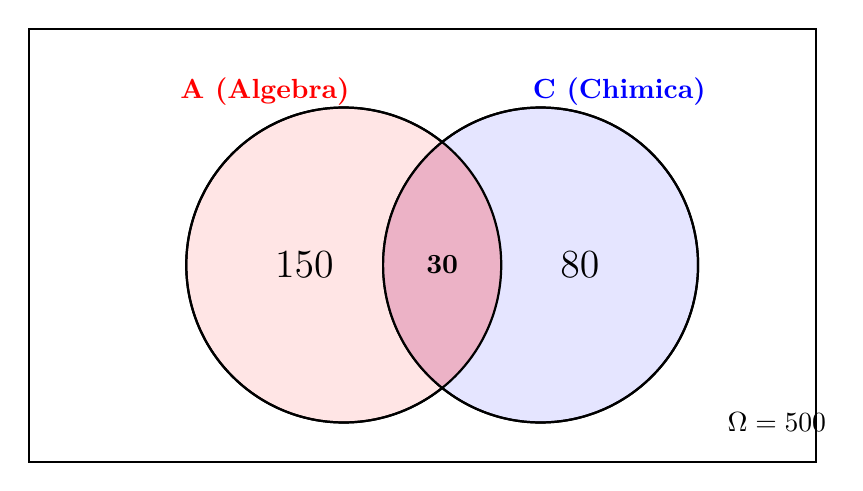
\begin{tikzpicture}
    % Rettangolo Universo
    \draw[thick] (-4,-2.5) rectangle (6,3);
    \node at (5.5,-2) {$\Omega = 500$};
    
    % Cerchio A (Algebra)
    \draw[thick, fill=red!10] (0,0) circle (2cm);
    \node[red, font=\bfseries] at (-1, 2.2) {A (Algebra)};
    
    % Cerchio C (Chimica)
    \draw[thick, fill=blue!10] (2.5,0) circle (2cm);
    \node[blue, font=\bfseries] at (3.5, 2.2) {C (Chimica)};
    
    % Intersezione
    \begin{scope}
        \clip (0,0) circle (2cm);
        \fill[purple!30] (2.5,0) circle (2cm);
    \end{scope}
    \draw[thick] (0,0) circle (2cm); % Ridisegna contorno A
    \draw[thick] (2.5,0) circle (2cm); % Ridisegna contorno C
    
    % Etichette Numeriche
    % Solo Algebra: 150 tot - 30 inters = 120
    \node[font=\Large] at (-0.5,0) {150}; 
    
    % Intersezione
    \node[font=\Large, font=\bfseries] at (1.25,0) {30};
    
    % Solo Chimica: 80 tot - 30 inters = 50
    \node[font=\Large] at (3,0) {80};
    
\end{tikzpicture}
\end{center}

\subsubsection*{Soluzione}

\paragraph{(a) Probabilità semplice: $\mathbb{P}(A)$}
La domanda è: \emph{Qual è la probabilità che uno studente scelto a caso studi Algebra?}
\\Qui lo spazio campionario è l'intera scuola ($\Omega$). Non abbiamo informazioni aggiuntive, quindi usiamo il totale degli studenti come denominatore.

\[
\mathbb{P}(A) = \frac{\text{Studenti di Algebra}}{\text{Totale studenti}} = \frac{150}{500} = \frac{3}{10} = 30\%
\]

\paragraph{(b) Probabilità condizionata: $\mathbb{P}(C \mid A)$}
La domanda è: \emph{Sapendo che lo studente studia Algebra, qual è la probabilità che studi anche Chimica?}
\\L'informazione ``studia Algebra'' riduce il nostro universo (\textbf{restrizione dello spazio campionario}). Ignoriamo i 500 totali; ora contano solo i 150 studenti di Algebra.
\\Tra questi 150, quelli che fanno anche Chimica (l'intersezione) sono 30.
\\Domandiamoci: Quanti studenti che studiano chimica studiano anche algebra?

\[
\mathbb{P}(C \mid A) = \frac{\text{Studenti (Algebra e Chimica)}}{\text{Studenti di Algebra}} = \frac{30}{150} = \frac{1}{5} = 20\%
\]
\emph{Nota: L'informazione ha corretto l'aspettativa base di Chimica (che sarebbe $80/500 = 16\%$) portandola al $20\%$.}

\paragraph{(c) Probabilità condizionata inversa: $\mathbb{P}(A \mid C)$}
La domanda è: \emph{Sapendo che lo studente studia Chimica, qual è la probabilità che studi anche Algebra?}
\\Ora la condizione restringe l'universo ai soli 80 studenti di Chimica.
\\Tra questi 80, quelli che fanno anche Algebra sono sempre gli stessi 30 (l'intersezione è commutativa).

\[
\mathbb{P}(A \mid C) = \frac{\text{Studenti (Algebra e Chimica)}}{\text{Studenti di Chimica}} = \frac{30}{80} = \frac{3}{8} = 37,5\%
\]
\emph{Nota: L'informazione ha corretto l'aspettativa base di Algebra dal $30\%$ al $37,5\%$.}

\paragraph{Conclusione}
In entrambi i casi condizionati (b) e (c), il numeratore rimane lo stesso (l'intersezione $30$), ma il denominatore cambia in base all'evento che sappiamo essere già accaduto, modificando così la probabilità finale.

\end{esempio}

\section{Legge della Probabilità Totale}

Il teorema permette di calcolare la probabilità di un evento $A$ sfruttando una partizione dello spazio campionario $\Omega$.

\subsection{Ipotesi: La Partizione}

Sia $\{E_i\}_{i=1}^M$ una famiglia di insiemi che costituisce una \textbf{partizione} di $\Omega$. Affinché sia una partizione, devono valere due condizioni fondamentali:

\begin{enumerate}
    \item \textbf{Esaustività:} L'unione degli insiemi copre l'intero spazio campionario.
    \[ \bigcup_{i=1}^M E_i = \Omega \]
    
    \item \textbf{Disgiunzione a coppie:} Gli insiemi non hanno elementi in comune tra loro.
    \[ E_i \cap E_j = \emptyset, \quad \forall i \neq j \]
\end{enumerate}

\subsection{Scomposizione dell'evento A}

Consideriamo un evento generico $A \subseteq \Omega$.
\\Possiamo riscrivere $A$ come l'intersezione di se stesso con l'intero spazio campionario $\Omega$ (poiché intersecare con l'insieme universo non cambia l'insieme):
\[ A = A \cap \Omega \]

Sostituendo $\Omega$ con la definizione di partizione (punto 1), otteniamo:
\[ A = A \cap \left( \bigcup_{i=1}^M E_i \right) \]

Applicando la \textbf{proprietà distributiva} dell'intersezione rispetto all'unione, portiamo l'intersezione dentro la sommatoria insiemistica:
\[ A = \bigcup_{i=1}^M (A \cap E_i) \]

\paragraph{Nota fondamentale}
Poiché gli insiemi $E_i$ sono disgiunti tra loro, anche le loro intersezioni con $A$ (ovvero i sottoinsiemi $A \cap E_i$) sono disgiunte a coppie.
\[ (A \cap E_i) \cap (A \cap E_j) = \emptyset, \quad \forall i \neq j \]

\subsection{Passaggio alla Probabilità (Assioma di Additività)}

Calcoliamo ora la probabilità di $A$, ovvero $\mathbb{P}(A)$.
\\Sfruttando la scomposizione appena trovata:
\[ \mathbb{P}(A) = \mathbb{P}\left( \bigcup_{i=1}^M (A \cap E_i) \right) \]

Per il \textbf{terzo assioma di Kolmogorov} (additività finita), poiché gli eventi $(A \cap E_i)$ sono disgiunti, la probabilità dell'unione è uguale alla somma delle probabilità:
\[ \mathbb{P}(A) = \sum_{i=1}^M \mathbb{P}(A \cap E_i) \]

\subsection{Applicazione della Probabilità Condizionata}

Dalla definizione di probabilità condizionata sappiamo che:
\[ \mathbb{P}(A \mid E_i) = \frac{\mathbb{P}(A \cap E_i)}{\mathbb{P}(E_i)} \quad (\text{con } \mathbb{P}(E_i) > 0) \]

Invertendo la formula, possiamo esprimere la probabilità congiunta come prodotto:
\[ \mathbb{P}(A \cap E_i) = \mathbb{P}(A \mid E_i) \cdot \mathbb{P}(E_i) \]

Sostituendo quest'ultima espressione nella sommatoria del punto 3, otteniamo la formula della Legge della Probabilità Totale:

\begin{equation}
\boxed{\mathbb{P}(A) = \sum_{i=1}^M \mathbb{P}(A \mid E_i)\mathbb{P}(E_i)}
\end{equation}

\paragraph{Interpretazione analitica}
Il teorema afferma che la probabilità marginale di $A$ è una \textbf{media ponderata} delle probabilità condizionate $\mathbb{P}(A \mid E_i)$, dove i pesi sono dati dalle probabilità degli eventi della partizione $\mathbb{P}(E_i)$.

\section{Indipendenza Stocastica (Eventi Indipendenti)}

Due eventi $A$ e $B$ si dicono indipendenti quando l'accadere di uno non modifica in alcun modo la probabilità che accada l'altro. In termini semplici: l'informazione su un evento non aggiunge nulla alla conoscenza dell'altro.

\subsection{1. Definizione Formale tramite Probabilità Condizionata}

Matematicamente, l'indipendenza si traduce nel fatto che la probabilità condizionata è uguale alla probabilità non condizionata (marginale).
\\Due eventi $A$ e $B$ sono indipendenti se e solo se:

\[
\mathbb{P}(A \mid B) = \mathbb{P}(A)
\]
(La probabilità di $A$ dato $B$ è uguale alla probabilità di $A$: sapere $B$ non serve a nulla).

E analogamente:
\[
\mathbb{P}(B \mid A) = \mathbb{P}(B)
\]

\subsection{2. La Regola del Prodotto (Fattorizzazione)}

Questa è la proprietà più usata negli esercizi per verificare l'indipendenza.
\\Partendo dalla definizione di probabilità condizionata $\mathbb{P}(A \mid B) = \frac{\mathbb{P}(A \cap B)}{\mathbb{P}(B)}$ e ponendo $\mathbb{P}(A \mid B) = \mathbb{P}(A)$, otteniamo la Legge della Probabilità Composta per eventi indipendenti:

\begin{equation}
\boxed{\mathbb{P}(A \cap B) = \mathbb{P}(A) \cdot \mathbb{P}(B)}
\end{equation}

\paragraph{Importante}
Questa formula vale \textbf{solo} se gli eventi sono indipendenti.
\begin{itemize}
    \item Se $\mathbb{P}(A \cap B) = \mathbb{P}(A)\mathbb{P}(B) \implies$ Sono \textbf{Indipendenti}.
    \item Se $\mathbb{P}(A \cap B) \neq \mathbb{P}(A)\mathbb{P}(B) \implies$ Sono \textbf{Dipendenti} (cioè uno influenza l'altro).
\end{itemize}

\subsection{3. Esempio: Lancio di un dado due volte}

Consideriamo l'esperimento di lanciare un dado ``onesto'' due volte consecutive.
\begin{itemize}
    \item \textbf{Evento 1:} Esce il numero $i$ al primo lancio. $\mathbb{P}(\{i\}) = \frac{1}{6}$.
    \item \textbf{Evento 2:} Esce il numero $j$ al secondo lancio. $\mathbb{P}(\{j\}) = \frac{1}{6}$.
\end{itemize}

Il dado non ha ``memoria'': il risultato del secondo lancio non dipende dal primo.
\\La probabilità di ottenere la coppia specifica $\{i, j\}$ (intersezione dei due eventi) è il prodotto delle singole probabilità:

\[
\mathbb{P}(\{i, j\}) = \mathbb{P}(\{i\}) \cdot \mathbb{P}(\{j\}) = \frac{1}{6} \cdot \frac{1}{6} = \frac{1}{36}
\]

\paragraph{Nota Bene: Indipendenti vs Disgiunti (Attenzione all'errore comune)}

Non confondere eventi \textbf{Indipendenti} con eventi \textbf{Disgiunti} (o incompatibili).

\begin{itemize}
    \item \textbf{Disgiunti ($A \cap B = \emptyset$):} Se accade $A$, $B$ \emph{non può} accadere. Quindi si influenzano tantissimo! Se so che è successo $A$, la probabilità di $B$ diventa immediatamente 0. Sono fortemente \textbf{dipendenti}.
    
    \item \textbf{Indipendenti:} Se accade $A$, la probabilità di $B$ rimane invariata. Possono accadere insieme (l'intersezione non è vuota, ma ha probabilità pari al prodotto delle singole probabilità).
\end{itemize}

\subsection{Algebra di eventi}
Un'algebra di eventi (o Algebra di sottoinsiemi di $\Omega$) è la collezione di tutti gli "eventi osservabili" o "misurabili" su cui ha senso calcolare una probabilità, garantendo che le operazioni logiche (NOT, OR, AND) non ci portino fuori da questa collezione.

Questa struttura algebrica può essere formalizzata dalla sestupla:
\[ (\mathcal{E}, \cup, \cap, ^c, \Omega, \emptyset) \]
dove $\mathcal{E}$ è una famiglia di sottoinsiemi dello spazio campionario $\Omega$.

Affinché $\mathcal{E}$ sia un'algebra, richiediamo che soddisffi le seguenti proprietà:
\begin{enumerate}
    \item $\mathcal{E}$ sia chiusa rispetto all'operazione di unione finita (se $A, B \in \mathcal{E} \implies A \cup B \in \mathcal{E}$).
    \item $\mathcal{E}$ sia chiusa rispetto all'operazione di complementazione (se $A \in \mathcal{E} \implies A^c \in \mathcal{E}$).
\end{enumerate}

Da queste due proprietà deriva automaticamente che l'insieme universo $\Omega$ e l'insieme vuoto $\emptyset$ appartengono all'algebra. Infatti, poiché $A \in \mathcal{E} \implies A^c \in \mathcal{E}$, osserviamo che:
\[ A \cup A^c = \Omega \quad \text{(L'evento certo appartiene a } \mathcal{E}) \]
E per complementazione:
\[ \Omega^c = \emptyset \quad \text{(L'evento impossibile appartiene a } \mathcal{E}) \]

\paragraph{Estensione alla $\sigma$-algebra}
Se richiediamo che la famiglia $\mathcal{E}$ sia chiusa non solo rispetto all'unione finita, ma anche rispetto all'\textbf{unione numerabile} (infinita), allora $\mathcal{E}$ si definisce una \textbf{$\sigma$-algebra}:
\[
\text{Se } A_1, A_2, \dots \in \mathcal{E} \implies \bigcup_{i=1}^{\infty} A_i \in \mathcal{E}
\]

Nota: Se lo spazio campionario $\Omega$ è finito, ogni unione numerabile si riduce a un'unione finita. Di conseguenza, nel caso finito, le definizioni di Algebra e $\sigma$-algebra coincidono.
\clearpage
Dalle definizioni di chiusura rispetto all'unione e alla complementazione, derivano automaticamente altre proprietà fondamentali per l'algebra di eventi $\mathcal{E}$:

\begin{itemize}
    \item \textbf{Chiusura rispetto all'intersezione:} \\
    Se $A, B \in \mathcal{E}$, allora $A \cap B \in \mathcal{E}$. \\
    \textit{Dimostrazione:} Utilizzando le leggi di De Morgan, possiamo scrivere l'intersezione come:
    \[ A \cap B = (A^c \cup B^c)^c \]
    Poiché $A, B \in \mathcal{E}$, i loro complementari $A^c, B^c \in \mathcal{E}$. Di conseguenza, la loro unione $(A^c \cup B^c) \in \mathcal{E}$ e, infine, il complemento di quest'ultima appartiene ancora a $\mathcal{E}$.

    \item \textbf{Chiusura rispetto alla differenza insiemistica:} \\
    Se $A, B \in \mathcal{E}$, allora $A \setminus B \in \mathcal{E}$. \\
    \textit{Dimostrazione:} Possiamo riscrivere la differenza come:
    \[ A \setminus B = A \cap B^c \]
    Poiché abbiamo appena dimostrato che l'algebra è chiusa rispetto all'intersezione e sappiamo che $B^c \in \mathcal{E}$, la proprietà è verificata.

    \item \textbf{Algebra minima (o generata da un evento):} \\
    Se $A$ è un evento qualsiasi, la minima algebra che contiene $A$ è l'insieme:
    \[ \mathcal{E}_A = \{A, A^c, \Omega, \emptyset\} \]
    Infatti:
    \begin{itemize}
        \item[$\dagger$] $A^c$ deve appartenere a $\mathcal{E}_A$ per la proprietà di chiusura rispetto alla complementazione;
        \item[$\dagger$] $\Omega = A \cup A^c$ deve appartenere a $\mathcal{E}_A$ per la proprietà di chiusura rispetto all'unione;
        \item[$\dagger$] $\emptyset = \Omega^c$ deve appartenere a $\mathcal{E}_A$ per la proprietà di chiusura rispetto alla complementazione.
    \end{itemize}
\end{itemize}

\subsection{Spazi di Probabilità}
Uno spazio di probabilità è il modello matematico completo che descrive un esperimento casuale.
Mettiamo insieme quanto detto fino ad ora:
Alla nostra struttura algebrica dobbiamo aggiungere un pezzo: La misura (quanto è probabile che accada qualcosa?).

Formalmente uno spazio di probabilità è una terna formata da: $(\Omega, \mathcal{E}, \mathbb{P})$
dove:

\paragraph{$\Omega$ (Spazio Campionario)}
È l'insieme di tutti i possibili esiti elementari (l'insieme ``sostegno'').
\begin{itemize}
    \item \textit{Esempio:} Nel lancio di un dado, $\Omega=\{1, 2, 3, 4, 5, 6\}$.
\end{itemize}

\paragraph{$\mathcal{E}$ ($\sigma$-algebra degli eventi)}
(Come definito nella sezione precedente).

\paragraph{$\mathbb{P}$ (Misura di Probabilità)}
$\mathbb{P}$ è una funzione: $\mathbb{P}: \mathcal{E} \to [0,1]$ (appartenente a $\mathbb{R}$).
Questa funzione deve soddisfare i 3 \textbf{assiomi di Kolmogorov}:

La funzione $\mathbb{P}$ definisce uno spazio di probabilità $\iff$

\begin{enumerate}
    \item \textbf{Non negativa:} per ogni evento $A \in \mathcal{E}$ la probabilità è un numero non negativo: 
    \[ \mathbb{P}(A) \ge 0 \quad \forall A \in \mathcal{E}; \]
    
    \item \textbf{Normalizzazione (o dell'Evento Certo):} La probabilità dell'intero spazio campionario è 1 (il 100\%):
    \[ \mathbb{P}(\Omega) = 1 \]
    \item \textbf{Sub-additività, cioè:} \\
    $A$ e $B$ incompatibili $(A \cap B = \emptyset) \implies \mathbb{P}(A \cup B) = \mathbb{P}(A) + \mathbb{P}(B)$
    \\\\e 3.1 \textbf{$\sigma$-additività (Additività numerabile):}
    Se abbiamo una sequenza infinita (numerabile) di eventi $A_1, A_2, \dots \in \mathcal{E}$ che sono \textbf{a due a due disgiunti} (cioè $A_i \cap A_j = \emptyset$ per ogni $i \neq j$), allora la probabilità della loro unione è la somma delle loro probabilità:
    \[ \mathbb{P}\left( \bigcup_{i=1}^{\infty} A_i \right) = \sum_{i=1}^{\infty} \mathbb{P}(A_i) \]
    \textit{(Se lo spazio è finito, basta l'additività finita).}
\end{enumerate}

La terna $(\Omega, \mathcal{E}, \mathbb{P})$ si definisce \textbf{Spazio di Probabilità}.

Questa definizione collega l'astrazione algebrica alla misura.
In matematica, uno \textbf{Spazio di Probabilità} è un caso specifico di uno \textbf{Spazio di Misura}.

\begin{itemize}
    \item Uno spazio di misura è una terna $(\Omega, \mathcal{E}, \mu)$ dove $\mu(\Omega)$ può essere qualsiasi numero (anche infinito, come la lunghezza di una retta).
    \item Uno spazio di probabilità è uno spazio di misura ``finito'' e ``normalizzato'' dove la misura totale deve fare esattamente 1.
\end{itemize}

\paragraph{Conseguenze degli Assiomi}

\begin{itemize}
    \item[$\dagger$] \textbf{Eventi complementari:} \\
    Poiché $A$ e $\overline{A}$ sono disgiunti e la loro unione è l'evento certo $\Omega$:
    \[
    \mathbb{P}(\Omega) = \mathbb{P}(A \cup \overline{A}) = \mathbb{P}(A) + \mathbb{P}(\overline{A}) = 1 \implies \mathbb{P}(\overline{A}) = 1 - \mathbb{P}(A)
    \]

    \item[$\dagger$] \textbf{Sottrazione tra insiemi:} \\
    Possiamo scomporre l'evento $A$ intersecandolo con l'universo partizionato da $B$:
    \[
    A = A \cap \Omega = A \cap (B \cup \overline{B}) = (A \cap B) \cup (A \cap \overline{B})
    \]
    Siccome $(A \cap B)$ e $(A \cap \overline{B})$ sono incompatibili (disgiunti), allora per l'additività:
    \[
    \mathbb{P}(A) = \mathbb{P}(A \cap B) + \mathbb{P}(A \cap \overline{B})
    \]
    Isolando il termine della differenza, ritroviamo la proprietà:
    \[
    \mathbb{P}(A \cap \overline{B}) = \mathbb{P}(A \setminus B) = \mathbb{P}(A) - \mathbb{P}(A \cap B)
    \]

    \item[$\dagger$] \textbf{Unione di eventi non incompatibili:} \\
    Se $A \cap B \neq \emptyset$, non possiamo sommare semplicemente le probabilità. Osserviamo preliminarmente che possiamo scrivere l'unione come somma di insiemi disgiunti:
    \[ A \cup B = A \cup (B \cap \overline{A}) \]
    Per cui, calcolando la probabilità:
    \[
    \mathbb{P}(A \cup B) = \mathbb{P}(A) + \underbrace{\mathbb{P}(B \cap \overline{A})}_{=\mathbb{P}(B)-\mathbb{P}(A \cap B)} = \mathbb{P}(A) + \mathbb{P}(B) - \mathbb{P}(A \cap B)
    \]

    \item[$\dagger$] \textbf{Se due eventi sono indipendenti allora anche i loro complementi sono indipendenti:} \\
    Due eventi $A$ e $B$ sono indipendenti, quindi vale la relazione:
\[ \mathbb{P}(A \cap B) = \mathbb{P}(A) \cdot \mathbb{P}(B) \]
    \[ \mathbb{P}(\overline{A} \cap \overline{B}) = \mathbb{P}(\overline{A}) \cdot \mathbb{P}(\overline{B}) \]
\end{itemize}

